% Generated from canonical MDX by scripts/generate-doc-artifacts.py.
% Options for packages loaded elsewhere
\PassOptionsToPackage{unicode}{hyperref}
\PassOptionsToPackage{hyphens}{url}
\PassOptionsToPackage{dvipsnames,svgnames,x11names}{xcolor}
%
\documentclass[
  10pt,
  letterpaper,
]{article}
\usepackage{amsmath,amssymb}
\usepackage{iftex}
\ifPDFTeX
  \usepackage[T1]{fontenc}
  \usepackage[utf8]{inputenc}
  \usepackage{textcomp} % provide euro and other symbols
\else % if luatex or xetex
  \usepackage{unicode-math} % this also loads fontspec
  \defaultfontfeatures{Scale=MatchLowercase}
  \defaultfontfeatures[\rmfamily]{Ligatures=TeX,Scale=1}
\fi
\usepackage{lmodern}
\ifPDFTeX\else
  % xetex/luatex font selection
  \setmainfont[]{DejaVu Serif}
  \setmonofont[]{DejaVu Sans Mono}
\fi
% Use upquote if available, for straight quotes in verbatim environments
\IfFileExists{upquote.sty}{\usepackage{upquote}}{}
\IfFileExists{microtype.sty}{% use microtype if available
  \usepackage[]{microtype}
  \UseMicrotypeSet[protrusion]{basicmath} % disable protrusion for tt fonts
}{}
\makeatletter
\@ifundefined{KOMAClassName}{% if non-KOMA class
  \IfFileExists{parskip.sty}{%
    \usepackage{parskip}
  }{% else
    \setlength{\parindent}{0pt}
    \setlength{\parskip}{6pt plus 2pt minus 1pt}}
}{% if KOMA class
  \KOMAoptions{parskip=half}}
\makeatother
\usepackage{xcolor}
\usepackage[margin=0.75in]{geometry}
\usepackage{color}
\usepackage{fancyvrb}
\newcommand{\VerbBar}{|}
\newcommand{\VERB}{\Verb[commandchars=\\\{\}]}
\DefineVerbatimEnvironment{Highlighting}{Verbatim}{commandchars=\\\{\}}
% Add ',fontsize=\small' for more characters per line
\newenvironment{Shaded}{}{}
\newcommand{\AlertTok}[1]{\textcolor[rgb]{1.00,0.00,0.00}{\textbf{#1}}}
\newcommand{\AnnotationTok}[1]{\textcolor[rgb]{0.38,0.63,0.69}{\textbf{\textit{#1}}}}
\newcommand{\AttributeTok}[1]{\textcolor[rgb]{0.49,0.56,0.16}{#1}}
\newcommand{\BaseNTok}[1]{\textcolor[rgb]{0.25,0.63,0.44}{#1}}
\newcommand{\BuiltInTok}[1]{\textcolor[rgb]{0.00,0.50,0.00}{#1}}
\newcommand{\CharTok}[1]{\textcolor[rgb]{0.25,0.44,0.63}{#1}}
\newcommand{\CommentTok}[1]{\textcolor[rgb]{0.38,0.63,0.69}{\textit{#1}}}
\newcommand{\CommentVarTok}[1]{\textcolor[rgb]{0.38,0.63,0.69}{\textbf{\textit{#1}}}}
\newcommand{\ConstantTok}[1]{\textcolor[rgb]{0.53,0.00,0.00}{#1}}
\newcommand{\ControlFlowTok}[1]{\textcolor[rgb]{0.00,0.44,0.13}{\textbf{#1}}}
\newcommand{\DataTypeTok}[1]{\textcolor[rgb]{0.56,0.13,0.00}{#1}}
\newcommand{\DecValTok}[1]{\textcolor[rgb]{0.25,0.63,0.44}{#1}}
\newcommand{\DocumentationTok}[1]{\textcolor[rgb]{0.73,0.13,0.13}{\textit{#1}}}
\newcommand{\ErrorTok}[1]{\textcolor[rgb]{1.00,0.00,0.00}{\textbf{#1}}}
\newcommand{\ExtensionTok}[1]{#1}
\newcommand{\FloatTok}[1]{\textcolor[rgb]{0.25,0.63,0.44}{#1}}
\newcommand{\FunctionTok}[1]{\textcolor[rgb]{0.02,0.16,0.49}{#1}}
\newcommand{\ImportTok}[1]{\textcolor[rgb]{0.00,0.50,0.00}{\textbf{#1}}}
\newcommand{\InformationTok}[1]{\textcolor[rgb]{0.38,0.63,0.69}{\textbf{\textit{#1}}}}
\newcommand{\KeywordTok}[1]{\textcolor[rgb]{0.00,0.44,0.13}{\textbf{#1}}}
\newcommand{\NormalTok}[1]{#1}
\newcommand{\OperatorTok}[1]{\textcolor[rgb]{0.40,0.40,0.40}{#1}}
\newcommand{\OtherTok}[1]{\textcolor[rgb]{0.00,0.44,0.13}{#1}}
\newcommand{\PreprocessorTok}[1]{\textcolor[rgb]{0.74,0.48,0.00}{#1}}
\newcommand{\RegionMarkerTok}[1]{#1}
\newcommand{\SpecialCharTok}[1]{\textcolor[rgb]{0.25,0.44,0.63}{#1}}
\newcommand{\SpecialStringTok}[1]{\textcolor[rgb]{0.73,0.40,0.53}{#1}}
\newcommand{\StringTok}[1]{\textcolor[rgb]{0.25,0.44,0.63}{#1}}
\newcommand{\VariableTok}[1]{\textcolor[rgb]{0.10,0.09,0.49}{#1}}
\newcommand{\VerbatimStringTok}[1]{\textcolor[rgb]{0.25,0.44,0.63}{#1}}
\newcommand{\WarningTok}[1]{\textcolor[rgb]{0.38,0.63,0.69}{\textbf{\textit{#1}}}}
\usepackage{longtable,booktabs,array}
\usepackage{calc} % for calculating minipage widths
% Correct order of tables after \paragraph or \subparagraph
\usepackage{etoolbox}
\makeatletter
\patchcmd\longtable{\par}{\if@noskipsec\mbox{}\fi\par}{}{}
\makeatother
% Allow footnotes in longtable head/foot
\IfFileExists{footnotehyper.sty}{\usepackage{footnotehyper}}{\usepackage{footnote}}
\makesavenoteenv{longtable}
\setlength{\emergencystretch}{3em} % prevent overfull lines
\providecommand{\tightlist}{%
  \setlength{\itemsep}{0pt}\setlength{\parskip}{0pt}}
\setcounter{secnumdepth}{5}
\ifLuaTeX
  \usepackage{selnolig}  % disable illegal ligatures
\fi
\usepackage{bookmark}
\IfFileExists{xurl.sty}{\usepackage{xurl}}{} % add URL line breaks if available
\urlstyle{same}
\hypersetup{
  pdftitle={FOS: The Digital Collectibles and Allocation Protocol},
  pdfauthor={FOS Project Documentation},
  colorlinks=true,
  linkcolor={blue},
  filecolor={Maroon},
  citecolor={Blue},
  urlcolor={Blue},
  pdfcreator={LaTeX via pandoc}}

\title{FOS: The Digital Collectibles and Allocation Protocol}
\usepackage{etoolbox}
\makeatletter
\providecommand{\subtitle}[1]{% add subtitle to \maketitle
  \apptocmd{\@title}{\par {\large #1 \par}}{}{}
}
\makeatother
\subtitle{Robinhood Chain / Base VRF and CCIP / Three-Plan Referral
Edition}
\author{FOS Project Documentation}
\date{October 12, 2026}

\usepackage{tikz}
\usepackage{float}
\usetikzlibrary{arrows.meta}
\setcounter{tocdepth}{1}
\emergencystretch=3em
\begin{document}
\maketitle

{
\hypersetup{linkcolor=}
\setcounter{tocdepth}{1}
\tableofcontents
\clearpage
}
\section{Executive Summary}\label{executive-summary}

FOS combines digital collectibles with protocol-defined distributions,
an independent single-level referral program, and authenticity
certificates. This edition updates the December 2025 whitepaper using
the supplied Persian project contract specification. User-facing
contracts move to Robinhood Chain. Base remains the specified
randomness-service chain through Chainlink VRF and CCIP.

This whitepaper explains the reported design. It is not an independent
contract audit, proof of a live bridge deployment, legal determination,
or promise of individual allocations. The documentation repository does
not contain the final Solidity sources or deployment ABI bundle.
Unverified operational contract addresses are not published here.

\subsection{Vision and mission}\label{vision-and-mission}

The project aims to make collectible participation and allocation
accounting visible through on-chain records rather than opaque operator
databases. Its practical goals are clear contract responsibilities,
explicit fee and reserve accounting, verifiable randomness, and
accessible user information. Owner configuration permissions and
cross-chain delivery dependencies are part of that design, not
exceptions to it.

\subsection{What changed in this
edition}\label{what-changed-in-this-edition}

\begin{itemize}
\tightlist
\item
  Robinhood Chain is the user transaction network; Base is retained for
  the specified VRF integration, connected through CCIP.
\item
  Referral has nominal \$2/\$5/\$10 plans; the direct referrer's active
  plan sets 50\%/60\%/82\% commission on registrations and upgrades.
\item
  Upgrades pay the current configured price difference and retain the
  original referrer.
\item
  Buddy/Samurai/Noble use 5\%/3\%/2\% admin fees and funded round pools
  of nominal \$1,425/\$6,305/\$12,250.
\item
  Free positions are funded from FOSNFT reserves; weighted uniqueness is
  at ticket level, not wallet level.
\item
  Draw completion is asynchronous; failed direct ETH payments become
  deferred claims.
\item
  Verify issues separate ERC-721 certificates and distinguishes
  existence from current validity.
\end{itemize}

\section{Market Context and Comparison
Limits}\label{market-context-and-comparison-limits}

The earlier whitepaper discussed digital collectibles, loyalty systems,
and trust in centralized promotions. Those motivations remain relevant
context, but historical Base adoption figures do not describe Robinhood
adoption. The existing 2025 research is historical and has not been
independently refreshed here.

Current economic statements in this edition follow the supplied
collection and referral arithmetic. Per-ticket pool fractions are 95\%,
97\%, and 98\% by collection, not a universal project-wide return rate.
Gas, oracle, bridge, audit, development, and compliance costs are not
assumed to vanish. Neither automation nor a terminology choice
determines regulatory classification.

The original references are retained in the unchanged historical PDF.
Current operational rules should be read from this edition and verified
against the actual deployment.

\section{Platform Infrastructure}\label{platform-infrastructure}

\subsection{Networks}\label{networks}

User-facing FOSNFT, Processor, Referral, and Verify interactions belong
on \textbf{Robinhood Chain}, not Base. Base serves the specified VRF
randomness integration, with CCIP transporting round requests and
results.

\begin{longtable}[]{@{}
  >{\raggedright\arraybackslash}p{(\columnwidth - 6\tabcolsep) * \real{0.2500}}
  >{\raggedleft\arraybackslash}p{(\columnwidth - 6\tabcolsep) * \real{0.2500}}
  >{\raggedright\arraybackslash}p{(\columnwidth - 6\tabcolsep) * \real{0.2500}}
  >{\raggedright\arraybackslash}p{(\columnwidth - 6\tabcolsep) * \real{0.2500}}@{}}
\toprule\noalign{}
\begin{minipage}[b]{\linewidth}\raggedright
Network
\end{minipage} & \begin{minipage}[b]{\linewidth}\raggedleft
Chain ID
\end{minipage} & \begin{minipage}[b]{\linewidth}\raggedright
Native currency
\end{minipage} & \begin{minipage}[b]{\linewidth}\raggedright
Role
\end{minipage} \\
\midrule\noalign{}
\endhead
\bottomrule\noalign{}
\endlastfoot
Robinhood Chain & 4663 & ETH & User-facing project network \\
Robinhood Chain Testnet & 46630 & Test ETH & Separate testing network \\
Base & Environment-specific & ETH & VRF service side of the specified
cross-chain design \\
\end{longtable}

The Robinhood IDs, currency, and URLs below are corroborated by the
public
\href{https://github.com/ethereum-lists/chains/blob/master/_data/chains/eip155-4663.json}{ethereum-lists
network registry}, with a
\href{https://github.com/ethereum-lists/chains/blob/master/_data/chains/eip155-46630.json}{separate
testnet entry}. This corroborates network metadata; it does not verify
FOS deployments or CCIP support.

\begin{itemize}
\tightlist
\item
  Mainnet RPC listed in the registry:
  \texttt{https://rpc.mainnet.chain.robinhood.com}
\item
  Mainnet explorer listed in the registry:
  \href{https://robinhoodchain.blockscout.com}{Robinhood Chain
  Blockscout}
\item
  Testnet RPC: \texttt{https://rpc.testnet.chain.robinhood.com/rpc}
\item
  Testnet explorer:
  \href{https://explorer.testnet.chain.robinhood.com}{Robinhood testnet
  explorer}
\item
  Official documentation linked by the registry:
  \href{https://docs.robinhood.com/chain}{Robinhood Chain documentation}
\end{itemize}

Verify the selected environment and live RPC chain ID before signing.
Never reuse Base or Base Sepolia addresses for a Robinhood transaction.
The Base environment used by the VRF integration must be confirmed
separately.

\subsection{ETH pricing and gas}\label{eth-pricing-and-gas}

The displayed dollar values are nominal product labels. On-chain ETH
prices and round settings are the transaction source of truth. Ordinary
mints require the exact configured price; free positions require zero
purchase value. Network gas still applies. ETH remains volatile, and
neither fixed gas costs nor USD-equivalent awards are guaranteed.

\subsection{Wallet access}\label{wallet-access}

Use an EVM wallet configured for the correct Robinhood network. MetaMask
and Coinbase Wallet are documented integration targets; connector
behavior must be verified in the deployed main application. This Next.js
repository hosts documentation and an AI assistant, not the minting
application itself.

The interface does not need a user's private key. Contracts nevertheless
hold round funds, reserved free-position contributions, and deferred
payments according to their rules. An interface described as
non-custodial does not mean that funds never enter a contract.

\subsection{Cross-chain visibility}\label{cross-chain-visibility}

Show Robinhood round status and transaction receipts separately from
Base VRF and CCIP delivery status. A successful last-mint receipt is not
evidence that the remote random result has arrived or that the
allocation transaction has completed.

\subsection{Network and draw
architecture}\label{network-and-draw-architecture}

\begin{figure}[H]
\centering
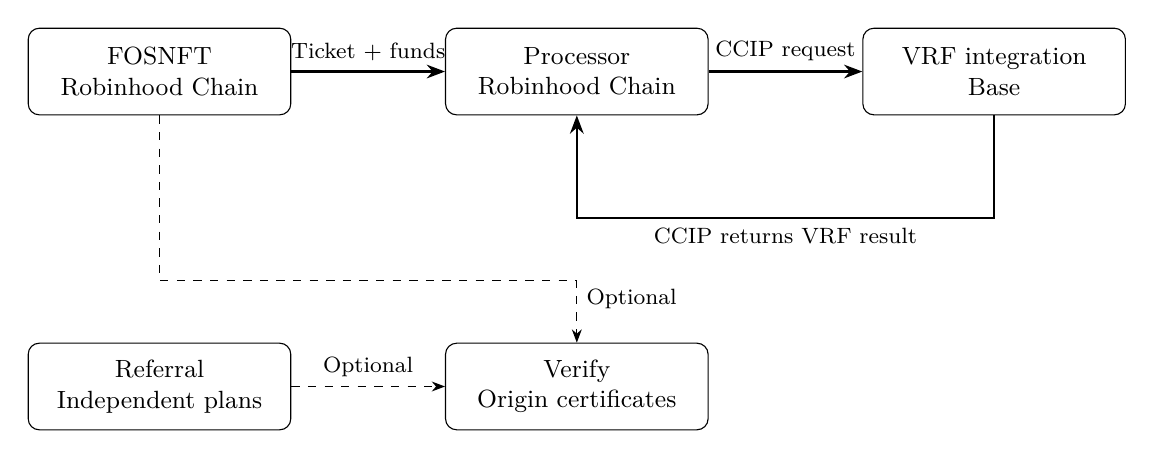
\begin{tikzpicture}[box/.style={draw,rounded corners,align=center,text width=3.1cm,minimum height=1.1cm,font=\small},>=Stealth]
\node[box] (mint) at (0,0) {FOSNFT\\Robinhood Chain};
\node[box] (processor) at (5.3,0) {Processor\\Robinhood Chain};
\node[box] (base) at (10.6,0) {VRF integration\\Base};
\draw[->,thick] (mint) -- node[above,font=\footnotesize] {Ticket + funds} (processor);
\draw[->,thick] (processor) -- node[above,font=\footnotesize] {CCIP request} (base);
\draw[->,thick] (base.south) -- ++(0,-1.3) -| node[pos=0.25,below,font=\footnotesize] {CCIP returns VRF result} (processor.south);
\node[box] (referral) at (0,-4) {Referral\\Independent plans};
\node[box] (verify) at (5.3,-4) {Verify\\Origin certificates};
\draw[->,dashed] (mint.south) -- ++(0,-2.1) -| node[pos=0.65,right,font=\footnotesize] {Optional} (verify.north);
\draw[->,dashed] (referral) -- node[above,font=\footnotesize] {Optional} (verify);
\end{tikzpicture}
\caption{Specified component boundaries. CCIP/VRF deployment and callback details require final implementation verification.}
\end{figure}

\section{Collection \& Protocol
Mechanics}\label{collection-protocol-mechanics}

\subsection{Minting}\label{minting}

Call \texttt{buyAndMint(lotteryType,\ tokenURI)} on FOSNFT on Robinhood
Chain. The documented type IDs are 3 (Buddy), 13 (Samurai), and 25
(Noble). A successful transaction mints an NFT, registers a ticket with
Processor, and sends the round's configured pool contribution to
Processor. Only FOSNFT may register tickets there. If Verify is
connected and FOSNFT is approved, a separate authenticity certificate is
also issued.

\subsection{Prices and accounting}\label{prices-and-accounting}

\begin{longtable}[]{@{}
  >{\raggedright\arraybackslash}p{(\columnwidth - 12\tabcolsep) * \real{0.1429}}
  >{\raggedleft\arraybackslash}p{(\columnwidth - 12\tabcolsep) * \real{0.1429}}
  >{\raggedleft\arraybackslash}p{(\columnwidth - 12\tabcolsep) * \real{0.1429}}
  >{\raggedleft\arraybackslash}p{(\columnwidth - 12\tabcolsep) * \real{0.1429}}
  >{\raggedleft\arraybackslash}p{(\columnwidth - 12\tabcolsep) * \real{0.1429}}
  >{\raggedleft\arraybackslash}p{(\columnwidth - 12\tabcolsep) * \real{0.1429}}
  >{\raggedleft\arraybackslash}p{(\columnwidth - 12\tabcolsep) * \real{0.1429}}@{}}
\toprule\noalign{}
\begin{minipage}[b]{\linewidth}\raggedright
Collection
\end{minipage} & \begin{minipage}[b]{\linewidth}\raggedleft
Type ID
\end{minipage} & \begin{minipage}[b]{\linewidth}\raggedleft
Nominal price
\end{minipage} & \begin{minipage}[b]{\linewidth}\raggedleft
Admin fee
\end{minipage} & \begin{minipage}[b]{\linewidth}\raggedleft
Admin per paid mint
\end{minipage} & \begin{minipage}[b]{\linewidth}\raggedleft
Pool contribution per ticket
\end{minipage} & \begin{minipage}[b]{\linewidth}\raggedleft
Full 500-ticket pool
\end{minipage} \\
\midrule\noalign{}
\endhead
\bottomrule\noalign{}
\endlastfoot
Buddy & 3 & \$3 & 5\% & \$0.15 & \$2.85 & \$1,425 \\
Samurai & 13 & \$13 & 3\% & \$0.39 & \$12.61 & \$6,305 \\
Noble & 25 & \$25 & 2\% & \$0.50 & \$24.50 & \$12,250 \\
\end{longtable}

Dollar amounts describe the product model, not a dollar-denominated
contract balance or guaranteed award. Payments and allocations use
native ETH. Read the configured on-chain price before sending a
transaction; the production USD-to-ETH conversion policy is not supplied
in the contract specification.

For each paid ticket:

\begin{Shaded}
\begin{Highlighting}[]
\NormalTok{adminCut = price * adminBps / 10000}
\NormalTok{prizeShare = price {-} adminCut}
\end{Highlighting}
\end{Shaded}

The admin share remains in FOSNFT. There is no additional admin
deduction from recipients' allocations. The amount sent to Processor
must equal the contribution stored for that round.

\subsection{Five gas-only positions}\label{five-gas-only-positions}

Positions \textbf{10, 100, 200, 300, and 400} are free in every round of
every collection. The buyer pays network gas but sends zero purchase
value. FOSNFT supplies the full pool contribution for each free ticket.
Admin withdrawals must preserve the reserve for remaining free
positions.

For a full round there are 495 paid positions and 5 funded free
positions. In nominal dollars:

\begin{longtable}[]{@{}
  >{\raggedright\arraybackslash}p{(\columnwidth - 10\tabcolsep) * \real{0.1667}}
  >{\raggedleft\arraybackslash}p{(\columnwidth - 10\tabcolsep) * \real{0.1667}}
  >{\raggedleft\arraybackslash}p{(\columnwidth - 10\tabcolsep) * \real{0.1667}}
  >{\raggedleft\arraybackslash}p{(\columnwidth - 10\tabcolsep) * \real{0.1667}}
  >{\raggedleft\arraybackslash}p{(\columnwidth - 10\tabcolsep) * \real{0.1667}}
  >{\raggedleft\arraybackslash}p{(\columnwidth - 10\tabcolsep) * \real{0.1667}}@{}}
\toprule\noalign{}
\begin{minipage}[b]{\linewidth}\raggedright
Collection
\end{minipage} & \begin{minipage}[b]{\linewidth}\raggedleft
Buyer purchase inflow
\end{minipage} & \begin{minipage}[b]{\linewidth}\raggedleft
Gross admin share from 495 paid positions
\end{minipage} & \begin{minipage}[b]{\linewidth}\raggedleft
Free-position funding
\end{minipage} & \begin{minipage}[b]{\linewidth}\raggedleft
Remaining admin amount
\end{minipage} & \begin{minipage}[b]{\linewidth}\raggedleft
Round pool
\end{minipage} \\
\midrule\noalign{}
\endhead
\bottomrule\noalign{}
\endlastfoot
Buddy & \$1,485 & \$74.25 & \$14.25 & \$60.00 & \$1,425 \\
Samurai & \$6,435 & \$193.05 & \$63.05 & \$130.00 & \$6,305 \\
Noble & \$12,375 & \$247.50 & \$122.50 & \$125.00 & \$12,250 \\
\end{longtable}

These calculations exclude gas, oracle/bridge costs, and any other
operating costs. The pool plus remaining admin amount equals the 495
buyers' total purchase payments.

\subsection{Weights and uniqueness}\label{weights-and-uniqueness}

Tickets 1--100 have two entries each in the selection pool; 101--500
have one. Positions 10 and 100 are both free and double-weighted. The
initial full-round selection pool contains 600 entries.

After a ticket is selected, all of its entries are removed. It cannot be
selected again in that round. A wallet holding multiple tickets may be
selected more than once through different tickets. Double weight is a
relative draw weight, not a guarantee of an award or a claim that every
final inclusion probability is exactly doubled.

\subsection{Green Eye and asynchronous
draw}\label{green-eye-and-asynchronous-draw}

The 500th collectible closes the round and is known as the Green Eye.

\begin{enumerate}
\def\labelenumi{\arabic{enumi}.}
\tightlist
\item
  FOSNFT registers ticket 500 with Processor on Robinhood Chain. That
  round closes to further tickets.
\item
  A round-specific randomness request is sent through Chainlink CCIP to
  the Base-side integration.
\item
  Chainlink VRF on Base produces verifiable randomness.
\item
  CCIP returns the result to the Robinhood-side integration.
\item
  Processor uses the returned randomness and ticket weights to select 17
  distinct winning tickets and process allocations.
\item
  After the draw completes, the next round of that collection starts
  automatically.
\end{enumerate}

The last mint starts this asynchronous sequence. Selection, transfers,
and the next round do \textbf{not} all finish in the last buyer's
transaction. Bridge contract names, callbacks, fee funding, supported
CCIP lane, and deployed bridge addresses must be checked against the
final implementation; this repository contains documentation, not those
Solidity contracts.

Do not assume a fixed 18× gas charge or an automatic fee reimbursement.
Each transaction has its own gas cost, and oracle/CCIP fees depend on
the final integration.

\subsection{Distribution and claims}\label{distribution-and-claims}

\begin{longtable}[]{@{}lrrr@{}}
\toprule\noalign{}
Group & Selected tickets & Share of pool & Per-ticket share \\
\midrule\noalign{}
\endhead
\bottomrule\noalign{}
\endlastfoot
Primary & 1 & 50\% & 50\% plus integer-rounding residue \\
Secondary & 6 & 30\% & 5\% \\
Tertiary & 10 & 20\% & 2\% \\
\end{longtable}

Processor attempts direct payment. A rejected payment is recorded in
\texttt{pendingWithdrawals} for a later \texttt{claim()} rather than
described as reverting every recipient's payment.

\subsection{Round settings}\label{round-settings}

Capacity, contribution per ticket, group counts/splits, and the number
of double-weighted positions are recorded at round start. Changes apply
to subsequent rounds; an empty active round may be updated where the
contract permits. The target capacity is 500; old 20-ticket settings
were tests.

The new specification does not establish the previously described
365-day \texttt{liquidatePool()} mechanism. Do not rely on that recovery
path unless it is confirmed in the final deployed contract.

\subsection{Asynchronous completion}\label{asynchronous-completion}

\begin{figure}[H]
\centering
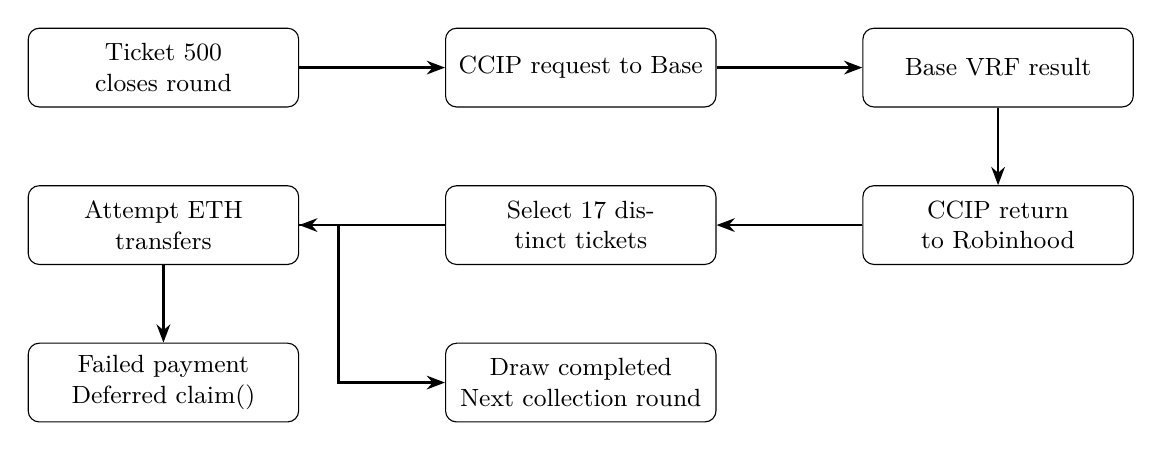
\begin{tikzpicture}[box/.style={draw,rounded corners,align=center,text width=3.2cm,minimum height=1cm,font=\small},>=Stealth]
\node[box] (full) at (0,0) {Ticket 500 closes round};
\node[box] (request) at (5.3,0) {CCIP request to Base};
\node[box] (vrf) at (10.6,0) {Base VRF result};
\node[box] (return) at (10.6,-2) {CCIP return to Robinhood};
\node[box] (select) at (5.3,-2) {Select 17 distinct tickets};
\node[box] (pay) at (0,-2) {Attempt ETH transfers};
\node[box] (claim) at (0,-4) {Failed payment\\Deferred claim()};
\node[box] (next) at (5.3,-4) {Draw completed\\Next collection round};
\draw[->,thick] (full) -- (request);
\draw[->,thick] (request) -- (vrf);
\draw[->,thick] (vrf) -- (return);
\draw[->,thick] (return) -- (select);
\draw[->,thick] (select) -- (pay);
\draw[->,thick] (pay) -- (claim);
\draw[->,thick] (pay.east) -- ++(.5,0) |- (next.west);
\end{tikzpicture}
\caption{Draw processing is separate from the last buyer's mint. Deferred claims remain owed after the draw is completed.}
\end{figure}

\section{Referral Program}\label{referral-program}

Referral is independent of NFT purchases and round allocations. Each
wallet registers once with a plan and, optionally, an existing
registered direct referrer.

\subsection{Plans and payment splits}\label{plans-and-payment-splits}

\begin{longtable}[]{@{}
  >{\raggedright\arraybackslash}p{(\columnwidth - 4\tabcolsep) * \real{0.3333}}
  >{\raggedleft\arraybackslash}p{(\columnwidth - 4\tabcolsep) * \real{0.3333}}
  >{\raggedleft\arraybackslash}p{(\columnwidth - 4\tabcolsep) * \real{0.3333}}@{}}
\toprule\noalign{}
\begin{minipage}[b]{\linewidth}\raggedright
Referrer's active plan
\end{minipage} & \begin{minipage}[b]{\linewidth}\raggedleft
Share of a direct referral's payment
\end{minipage} & \begin{minipage}[b]{\linewidth}\raggedleft
Admin share
\end{minipage} \\
\midrule\noalign{}
\endhead
\bottomrule\noalign{}
\endlastfoot
\$2 plan & 50\% & 50\% \\
\$5 plan & 60\% & 40\% \\
\$10 plan & 82\% & 18\% \\
\end{longtable}

The \textbf{referrer's own active plan at payment time} determines the
split, for both registration and upgrades. The buyer's plan determines
the payment amount, not the commission percentage. Without a referrer,
100\% goes to the admin. Dollar labels are nominal plan names; exact
payment is the configured ETH price.

\subsection{Register and share}\label{register-and-share}

Call \texttt{register(address\ referrer,\ uint256\ tier)} with tier
\textbf{2}, \textbf{5}, or \textbf{10} and exact configured payment. The
referrer must already be registered and cannot be the registering
wallet. Use the zero address to register without a referrer. The wallet
address identifies the referral link; \texttt{referredBy} records the
direct referrer permanently. A registration with a referrer increases
that referrer's \texttt{referralCount} by one.

\subsection{Upgrade by paying the
difference}\label{upgrade-by-paying-the-difference}

Registered users may call \texttt{upgrade(uint256\ newTier)} to move
2→5, 2→10, or 5→10. Downgrades and registering the same wallet again are
prohibited.

\begin{Shaded}
\begin{Highlighting}[]
\NormalTok{cost = tierPrice[newTier] {-} tierPrice[oldTier]}
\end{Highlighting}
\end{Shaded}

Read \texttt{getUpgradeCost} and the current prices before submitting.
Nominal differences are \$3, \$8, and \$5 respectively; actual payment
uses the current configured ETH difference. The upgrade is split with
the \textbf{same original direct referrer}. Without one, the full
upgrade payment goes to the admin.

\subsection{Example}\label{example}

\begin{enumerate}
\def\labelenumi{\arabic{enumi}.}
\tightlist
\item
  A has the \$2 plan. B registers through A with the \$2 plan. A
  receives 50\% of that payment, nominally \$1.
\item
  A upgrades to the \$10 plan.
\item
  B later upgrades from \$2 to \$5 and pays the nominal \$3 difference.
\item
  A now receives 82\% of that difference, nominally \$2.46; the admin
  receives \$0.54.
\end{enumerate}

If A had stayed on the \$2 plan, even a \$10 registration by B would use
A's 50\% rate. A's upgrade changes only subsequent payments; previous
payments are never recalculated.

\subsection{Single-level accounting}\label{single-level-accounting}

If A refers B and B refers C, A can receive a share of B's registration
and upgrades. C's registration and upgrades can pay B, not A. Plan
levels are price/commission plans, not additional generations of
referral compensation.

\subsection{Direct payment and deferred
claims}\label{direct-payment-and-deferred-claims}

The contract attempts direct ETH payment to the referrer. If that
transfer fails, it records the amount in \texttt{pendingWithdrawals};
the referrer uses \texttt{claim()} to collect it. \texttt{withdraw()} is
for the admin's available balance, not the referrer's claim function.

\subsection{Configuration and risk}\label{configuration-and-risk}

The owner can change plan prices, commission basis points, the admin
wallet, and the Verify connection. Price ordering must remain
\texttt{price(2)\ \textless{}\ price(5)\ \textless{}\ price(10)}.
Initial documented rates are 5000, 6000, and 8200 basis points out of
10000. Read current settings rather than assuming those values are
globally immutable.

Reported test prices of 0.0000002, 0.0000005, and 0.000001 ETH are test
settings, not production USD conversion rates. Referral participation
and any tax obligations remain the user's responsibility. Payments
depend on actual direct-referral activity and do not guarantee income.

See
\href{https://github.com/alirezaehteshampour/Fos-Doc/blob/main/content/docs/technical/referral-contract.mdx}{Referral
Contract} and
\href{https://github.com/alirezaehteshampour/Fos-Doc/blob/main/content/docs/technical/verification-contract.mdx}{Verify}.

\section{Smart Contracts}\label{smart-contracts}

\subsection{Contract suite}\label{contract-suite}

\begin{longtable}[]{@{}
  >{\raggedright\arraybackslash}p{(\columnwidth - 4\tabcolsep) * \real{0.3333}}
  >{\raggedright\arraybackslash}p{(\columnwidth - 4\tabcolsep) * \real{0.3333}}
  >{\raggedright\arraybackslash}p{(\columnwidth - 4\tabcolsep) * \real{0.3333}}@{}}
\toprule\noalign{}
\begin{minipage}[b]{\linewidth}\raggedright
Contract
\end{minipage} & \begin{minipage}[b]{\linewidth}\raggedright
Responsibility
\end{minipage} & \begin{minipage}[b]{\linewidth}\raggedright
Specified network
\end{minipage} \\
\midrule\noalign{}
\endhead
\bottomrule\noalign{}
\endlastfoot
\texttt{FOSNFT} & NFT mint, purchase payment, admin balance, free-ticket
reserve & Robinhood \\
\texttt{Processor} & Authorized ticket registration, round state, draw,
allocations & Robinhood \\
\texttt{Referral} & Registration, plans, upgrades, and direct-referral
payments & Robinhood \\
\texttt{Verify} & Separate ERC-721 certificates, origin registry,
validity status & Robinhood \\
VRF/CCIP integration & Carry round requests to Base and return VRF
results & Robinhood and Base \\
\end{longtable}

Only FOSNFT may register tickets in Processor. Referral is independent
of both contracts. Verify is optional and may be connected to FOSNFT and
Referral; Processor has no direct Verify connection in the supplied
structure.

\subsection{Three independent collection
types}\label{three-independent-collection-types}

\begin{longtable}[]{@{}
  >{\raggedright\arraybackslash}p{(\columnwidth - 12\tabcolsep) * \real{0.1429}}
  >{\raggedleft\arraybackslash}p{(\columnwidth - 12\tabcolsep) * \real{0.1429}}
  >{\raggedleft\arraybackslash}p{(\columnwidth - 12\tabcolsep) * \real{0.1429}}
  >{\raggedleft\arraybackslash}p{(\columnwidth - 12\tabcolsep) * \real{0.1429}}
  >{\raggedleft\arraybackslash}p{(\columnwidth - 12\tabcolsep) * \real{0.1429}}
  >{\raggedleft\arraybackslash}p{(\columnwidth - 12\tabcolsep) * \real{0.1429}}
  >{\raggedleft\arraybackslash}p{(\columnwidth - 12\tabcolsep) * \real{0.1429}}@{}}
\toprule\noalign{}
\begin{minipage}[b]{\linewidth}\raggedright
Collection
\end{minipage} & \begin{minipage}[b]{\linewidth}\raggedleft
Type ID
\end{minipage} & \begin{minipage}[b]{\linewidth}\raggedleft
Nominal price
\end{minipage} & \begin{minipage}[b]{\linewidth}\raggedleft
Admin fee
\end{minipage} & \begin{minipage}[b]{\linewidth}\raggedleft
Admin per paid mint
\end{minipage} & \begin{minipage}[b]{\linewidth}\raggedleft
Pool contribution per ticket
\end{minipage} & \begin{minipage}[b]{\linewidth}\raggedleft
Full 500-ticket pool
\end{minipage} \\
\midrule\noalign{}
\endhead
\bottomrule\noalign{}
\endlastfoot
Buddy & 3 & \$3 & 5\% & \$0.15 & \$2.85 & \$1,425 \\
Samurai & 13 & \$13 & 3\% & \$0.39 & \$12.61 & \$6,305 \\
Noble & 25 & \$25 & 2\% & \$0.50 & \$24.50 & \$12,250 \\
\end{longtable}

Dollar amounts describe the product model, not a dollar-denominated
contract balance or guaranteed award. Payments and allocations use
native ETH. Read the configured on-chain price before sending a
transaction; the production USD-to-ETH conversion policy is not supplied
in the contract specification.

All three target 500 tickets, with 17 selected tickets and 50/30/20
group allocation. There is no specified 100-round lifetime cap. Only the
initial weights and price labels are described here; per-round stored
settings and current on-chain prices control execution.

\subsection{Standards and authority}\label{standards-and-authority}

NFT/certificate documentation uses ERC-721. Do not infer ERC-721A,
ERC-1155, UUPS upgradeability, timelocks, or audit status from older
drafts. Referral owner controls include prices, split basis points,
admin wallet, and Verify connection. Verify owner controls include
approved minters, origin types, URI configuration, admin wallet, and
revocation.

\subsection{Deployment status}\label{deployment-status}

Robinhood Chain ID \textbf{4663} is reported by the supplied
specification and corroborated by the public network registry. The
specification provides incomplete addresses for some components and does
not supply the final Base-side bridge deployment. Accordingly this
reference does not publish operational FOS contract addresses, ABIs, RPC
credentials, or callback selectors. The named functions in individual
pages are specification references, not a replacement for a verified
ABI.

Genesis allowlist and growth campaign contracts remain design material
in the
\href{https://github.com/alirezaehteshampour/Fos-Doc/blob/main/content/docs/roadmap.mdx}{roadmap},
not confirmed members of this deployed four-contract suite.

\section{Verify Contract}\label{verify-contract}

Verify issues a separate ERC-721 certificate for supported official
events. It does not hold draw pools, run referrals, pay allocations, or
perform recipient selection.

\subsection{Origins}\label{origins}

\begin{longtable}[]{@{}rll@{}}
\toprule\noalign{}
ID & Constant & Use \\
\midrule\noalign{}
\endhead
\bottomrule\noalign{}
\endlastfoot
1 & \texttt{ORIGIN\_FREE\_MINT} & Free mint/campaign \\
2 & \texttt{ORIGIN\_LOTTERY} & Official FOSNFT round mint \\
3 & \texttt{ORIGIN\_STORY} & Story/content \\
4 & \texttt{ORIGIN\_ADMIN} & Manual admin issuance \\
5 & \texttt{ORIGIN\_REFERRAL} & Initial referral registration \\
\end{longtable}

Owner may define or enable/disable origin types using
\texttt{setOriginType}.

\subsection{Issuance and
authorization}\label{issuance-and-authorization}

\begin{itemize}
\tightlist
\item
  \texttt{adminMint(to,\ originTypeId,\ originId,\ uri)} is limited to
  owner or \texttt{adminWallet}.
\item
  \texttt{mintFromContract(to,\ originTypeId,\ originId,\ uri)} requires
  \texttt{approvedMinters{[}msg.sender{]}\ ==\ true}.
\item
  Owner authorizes a source with \texttt{setApprovedMinter}; the source
  sets its Verify connection with \texttt{setVerifyContract} under its
  own access controls.
\item
  Ordinary wallets cannot directly mint certificates.
\end{itemize}

FOSNFT's connected mint path issues origin type 2,
\texttt{originId\ =\ fosTokenId}, and the supplied URI. Referral's
connected registration path issues origin type 5, origin ID 0, and empty
URI. The specification does not issue a new certificate on referral
upgrade. Processor has no direct Verify integration in the supplied
design.

\subsection{Records}\label{records}

Token IDs begin at 1 and increase. \texttt{getNftInfo} exposes the
record; \texttt{totalMinted} gives the issuance count.

\begin{longtable}[]{@{}ll@{}}
\toprule\noalign{}
Field & Meaning \\
\midrule\noalign{}
\endhead
\bottomrule\noalign{}
\endlastfoot
\texttt{exists} & Record is registered \\
\texttt{active} & Current validity flag \\
\texttt{originType} & Origin category \\
\texttt{originContract} & Source contract or issuing caller \\
\texttt{originId} & Source event/asset identifier \\
\texttt{minter} & Initial recipient of the Verify NFT \\
\texttt{createdAt} & Issuance timestamp \\
\end{longtable}

\texttt{minter} is historical provenance, not current ownership. Read
ERC-721 ownership for the current holder. A certificate and its linked
FOSNFT are separate tokens.

\subsection{Check current status}\label{check-current-status}

\begin{longtable}[]{@{}rll@{}}
\toprule\noalign{}
Code & Status & Meaning \\
\midrule\noalign{}
\endhead
\bottomrule\noalign{}
\endlastfoot
0 & \texttt{NOT\_REGISTERED} & No record \\
1 & \texttt{OFFICIAL\_ACTIVE} & Official and currently active \\
2 & \texttt{OFFICIAL\_REVOKED} & Officially issued but revoked \\
\end{longtable}

\textbf{\texttt{isOfficial(tokenId)} checks existence only. It may
return true for a revoked token.} Interfaces must use \texttt{getStatus}
to display current validity.

Only owner may \texttt{revoke(tokenId,\ reasonCode)}. Revocation sets
\texttt{active\ =\ false}; it does not burn the NFT, transfer ownership,
or erase the record/history. Owner also manages approved minters,
origins, admin wallet, and URI configuration. \texttt{adminWallet} can
issue manual certificates but is not described as having owner-only
revocation authority.

\section{Main Application
Integration}\label{main-application-integration}

This Next.js repository is the documentation website. Older PHP paths
and wallet functions described in previous drafts are main-application
design references; their implementation is not present here. The
supplied contract update defines the following integration requirements.

\subsection{Wallet and network}\label{wallet-and-network}

Use Robinhood Chain for user transactions. Confirm \texttt{eth\_chainId}
matches the selected environment: mainnet 4663, testnet 46630. A Base
wallet balance or Base Sepolia chain ID is not a substitute. Obtain
RPC/explorer settings from the
\href{https://github.com/alirezaehteshampour/Fos-Doc/blob/main/content/docs/protocol/platform.mdx}{network
reference}, keeping environments separate.

\subsection{Mint interface}\label{mint-interface}

\begin{enumerate}
\def\labelenumi{\arabic{enumi}.}
\tightlist
\item
  Read collection type, round state, next ticket position, and exact
  configured ETH price.
\item
  Show nominal dollar labels separately from the required ETH
  transaction value.
\item
  For positions 10, 100, 200, 300, and 400, send zero purchase value and
  show the wallet's network gas estimate.
\item
  Submit \texttt{buyAndMint(lotteryType,\ tokenURI)} using the verified
  FOSNFT ABI and address.
\item
  Wait for a successful receipt, then refresh NFT/ticket data. Handle
  next-position races by refreshing and asking the user to sign a new
  transaction.
\item
  After ticket 500, display pending randomness/delivery until the
  cross-chain result and draw finalization are confirmed. Do not show a
  receipt as a completed payout.
\end{enumerate}

\subsection{Referral interface}\label{referral-interface}

Display current plan prices and commission rates from the contract.
Registration selects 2/5/10 and a valid direct referrer or zero address.
Upgrade options are only higher plans. Read \texttt{getUpgradeCost}
immediately before signing. Explain that the referrer's current plan
sets the split, and upgrades retain the original \texttt{referredBy}.

Show direct payments separately from \texttt{pendingWithdrawals}.
Referrers claim deferred ETH with \texttt{claim()}; admin
\texttt{withdraw()} is a different permissioned operation. Refresh
balances and plan status after confirmed receipts.

\subsection{Certificate interface}\label{certificate-interface}

Use Verify \texttt{getStatus} for current validity, \texttt{getNftInfo}
for origin details, and ERC-721 ownership for the current holder. Do not
call a revoked certificate active just because \texttt{isOfficial} is
true. Show original recipient separately from current owner.

\subsection{Leaderboard and campaigns}\label{leaderboard-and-campaigns}

The retained scoring design is referral +1, Buddy +2, Samurai +4, Noble
+6. Upgrade points, free-mint points, time-period ranking, and campaign
snapshots require the final app/indexer policy; the supplied contract
summary does not define all of them. \texttt{referralCount} and
\texttt{purchaseCount} are evidence for indexing, not a complete
specified leaderboard ABI.

\subsection{Operational views}\label{operational-views}

Show collection/round identifiers, Robinhood transaction hashes, pending
randomness, Base VRF request correlation, CCIP delivery state, selected
ticket IDs, attempted payments, and deferred claims. Filter logs by
chain and contract version; validate server responses and never ask
users for wallet private keys.

\section{Security \& Validation}\label{security-validation}

The supplied contract summary describes intended behavior. This
repository does not include Solidity sources, final ABIs, independent
audit reports, or evidence of a deployed VRF/CCIP lane. An audit,
timelock, multisig, or public retry function must not be claimed as
completed solely because it appeared in an older draft.

\subsection{Authority and funds}\label{authority-and-funds}

Referral owner can change prices, percentages, admin wallet, and Verify
connection. Verify owner controls authorized minters, origin types, URI
configuration, and revocation. Round settings are stored per round;
updates generally apply to future rounds, with permitted empty-round
updates. Publish real deployment roles and settings after verification.

The interface does not hold private keys, but contracts hold pool funds,
free-position reserves, and deferred payment liabilities. Native ETH is
volatile; automation does not remove smart-contract, network, or
regulatory risks.

\subsection{Required contract checks}\label{required-contract-checks}

\begin{itemize}
\tightlist
\item
  Registration: once per wallet, registered non-self referrer,
  zero-address path, exact payment, fixed \texttt{referredBy}.
\item
  Plans: strict price ordering, higher-plan upgrades only, current
  difference payment, referrer's current basis-point rate, no
  retroactive payment changes.
\item
  Funds: admin withdrawable balance excludes pending claims and FOSNFT's
  remaining free-ticket reserve.
\item
  Mint: only FOSNFT registers in Processor; exact contribution matching;
  independent collection rounds; free positions send zero purchase
  value.
\item
  Draw: double-weighted entries are removed together after selection; 17
  distinct tickets; repeated wallet recipients allowed; rounding residue
  assigned to primary.
\item
  Claims: failed pushes create correct liabilities; successful claims
  cannot repeat; transfers and claims resist reentrancy.
\item
  Verify: only approved issuers; origin linking; initial recipient
  versus current owner; revoked records remain official but inactive.
\end{itemize}

\subsection{Cross-chain checks}\label{cross-chain-checks}

Verify the actual CCIP-supported lane and configured routers/senders,
Base VRF environment and authorization, round/request correlation,
replay/stale response rejection, and exactly-once finalization. Test
delayed messages, failed request delivery, failed return delivery,
unavailable fee balances, and rejected recipient transfers.

Keep a pending round visible when randomness is unavailable. Do not
substitute block timestamps, \texttt{prevrandao}, or an
operator-selected result for the specified VRF design. A supported
retry/recovery path and the fee-funding policy must come from the final
implementation; the specification does not supply their callable ABI.

\subsection{Operational readiness}\label{operational-readiness}

Use verified full addresses and ABIs per environment, verify deployed
bytecode and role owners, check RPC chain ID, and monitor both chains.
Multisig/timelock protection, unit/invariant/fuzz tests, independent
audit, and privacy/access controls are recommended checks, not verified
features of this documentation repository.

No implemented 365-day liquidation guarantee, fixed 18× gas multiplier,
or no-risk claim is supported by the new contract summary.

\section{Community \& Growth}\label{community-growth}

\subsection{Recognition points}\label{recognition-points}

\begin{longtable}[]{@{}lr@{}}
\toprule\noalign{}
Action & Retained product score \\
\midrule\noalign{}
\endhead
\bottomrule\noalign{}
\endlastfoot
Valid direct referral registration & +1 \\
Buddy purchase & +2 \\
Samurai purchase & +4 \\
Noble purchase & +6 \\
\end{longtable}

Referral \texttt{referralCount} records direct registrations;
\texttt{purchaseCount{[}user{]}{[}type{]}} records collection activity.
The final app/indexer must define the ranking period, free-position
treatment, and tie-breaking. Referral upgrades change the plan and
commission rate, not the number of direct registrations; no new
upgrade-points rule is supplied.

Points are recognition metrics and are distinct from ticket selection
weight and referral commissions. Changing a referral plan does not
change the 1--100 double-weight rule in a draw.

\subsection{Genesis access}\label{genesis-access}

The retained roadmap proposes social verification through X, Discord,
YouTube, and Telegram, followed by a gas-only Genesis campaign for
eligible wallets. Actual launch dates, quotas, proof format, and
early-adopter benefits require campaign configuration. Genesis
eligibility must not be confused with the five ordinary round positions
that are free for the buyer.

\subsection{Growth campaign}\label{growth-campaign}

The planned separate campaign targets 5,000 users and a 30-day window,
with milestones and a top-three 50/30/20 split. Activation, funds,
deployment, and snapshots are not verified in the new contract summary.
Any funding must use available admin receipts after free-position
reserves and deferred user liabilities, never Processor's round pool.

See
\href{https://github.com/alirezaehteshampour/Fos-Doc/blob/main/content/docs/leaderboard.mdx}{Leaderboard},
\href{https://github.com/alirezaehteshampour/Fos-Doc/blob/main/content/docs/campaigns/index.mdx}{Campaigns},
\href{https://github.com/alirezaehteshampour/Fos-Doc/blob/main/content/docs/technical/campaign-contract.mdx}{campaign
design}, and the
\href{https://github.com/alirezaehteshampour/Fos-Doc/blob/main/content/docs/roadmap.mdx}{16-phase
roadmap}.

\section{Campaign \& Leaderboard
Design}\label{campaign-leaderboard-design}

The existing roadmap describes a separate growth campaign targeting
5,000 users, a 30-day window, milestones
\$20k/\$50k/\$100k/\$200k/\$500k/\$1M/\$2M, and 50/30/20 allocations to
the top three leaderboard accounts. The new contract specification does
not supply a campaign ABI, deployment, automatic activation proof, or
funded milestone state. Those remain design targets rather than live
guarantees.

\subsection{Funding boundary}\label{funding-boundary}

Only available admin funds may be committed to a campaign. Referral
admin receipts vary with the direct referrer's current \$2/\$5/\$10 plan
(50\%/40\%/18\%), or 100\% without a referrer. FOSNFT retains
collection-specific admin fees (5\%/3\%/2\%) but must reserve funding
for remaining free positions. Neither Processor pools nor deferred user
payments may be redirected as campaign revenue.

The new summary does not establish automatic routing to a campaign
vault. Publish that adapter/funding implementation before treating it as
active.

\subsection{Required campaign
specification}\label{required-campaign-specification}

Confirm the user-count source, activation authority/date, funding
window, incremental versus cumulative milestone funding, unique
snapshots, tie-break rules, rounding, claim eligibility, and recovery
behavior. A dollar milestone table is arithmetic, not evidence that
funds exist. Do not allocate the same funded balance again at multiple
milestones.

\subsection{Leaderboard}\label{leaderboard}

Retained product scoring is direct referral +1, Buddy purchase +2,
Samurai +4, Noble +6. The supplied summary provides
\texttt{referralCount} and \texttt{purchaseCount}; it does not establish
an on-chain global ranking or new points for referral upgrades. Verify
the app/indexer scoring and snapshots before making payout claims.

The campaign is separate from the 500-ticket round's 17-recipient draw.
Its planned three-account 50/30/20 split must not be confused with the
round's 1/6/10 ticket groups. See
\href{https://github.com/alirezaehteshampour/Fos-Doc/blob/main/content/docs/campaigns/growth.mdx}{Growth
Campaign}.

\section{Public Roadmap}\label{public-roadmap}

This is a development roadmap, not evidence that every feature has
launched. The current core specification places user-facing contracts on
Robinhood Chain, uses Base VRF through CCIP, and provides three referral
plans. Genesis/campaign contracts, launch status, and future features
need separate deployment confirmation.

\subsection{Phase 1 --- Community Introduction \& Whitelist Access
Program}\label{phase-1-community-introduction-whitelist-access-program}

This phase focuses on onboarding the first members of the ecosystem and
establishing a foundation of verified early supporters.

\begin{itemize}
\tightlist
\item
  Launch of the official website and ecosystem overview
\item
  Introduction of the FOS Protocol across the community channels
\item
  Opening of the Whitelist Access Program for early adopters
\item
  Participation-based tasks designed to help users learn about the
  platform and engage with the community
\item
  Whitelisted users receive priority access to the next participation
  stage
\end{itemize}

The Whitelist is a contribution-based access layer, not a financial
feature. It is designed to recognize genuine community participation
rather than speculation.

\subsection{Phase 2 --- Genesis Free-Mint Access (Whitelisted Users
Only)}\label{phase-2-genesis-free-mint-access-whitelisted-users-only}

Following the whitelist period, a dedicated Free-Mint Campaign is opened
exclusively to verified members.

\begin{itemize}
\tightlist
\item
  Whitelisted users may mint selected FOS Digital Collectibles
\item
  Participation requires network gas only (no protocol fee during this
  window)
\item
  Genesis assets and any Processor round eligibility must follow the
  separately published campaign configuration
\item
  The objective of this phase is to reward early contributors and
  establish the first active user base
\end{itemize}

This phase reinforces our principle of accessibility and loyalty
recognition, while remaining fully aligned with the protocol's
product-first architecture.

\subsection{Phase 3 --- Limited-Access Application Release (Stability
Validation
Stage)}\label{phase-3-limited-access-application-release-stability-validation-stage}

Before enabling full public access, the platform enters a restricted
availability period.

\begin{itemize}
\tightlist
\item
  The application is opened to a limited number of users
\item
  System performance, UX behavior, and contract execution are monitored
\item
  Feedback from real-world usage is incorporated
\item
  Technical and operational stability are validated
\end{itemize}

Only after the protocol demonstrates reliability in this controlled
environment does the platform proceed to full availability.

\subsection{Phase 4 --- Public Launch \& Open
Access}\label{phase-4-public-launch-open-access}

After stability validation, the protocol becomes publicly accessible.

\begin{itemize}
\tightlist
\item
  Full public access to the application
\item
  Ongoing onboarding of new participants
\item
  Continued growth through community-driven initiatives
\item
  Expansion of ecosystem transparency and engagement tools
\end{itemize}

Rounds follow their stored settings and asynchronous randomness
lifecycle. Authorized owner controls and oracle/bridge operations remain
part of the documented architecture.

\subsection{Phase 5 --- Growth Campaign (Activated at 5,000
Users)}\label{phase-5-growth-campaign-activated-at-5000-users}

Once the ecosystem reaches 5,000 verified participants, the protocol
activates a time-limited Growth Campaign Layer as defined in the
technical and economic documentation.

\begin{itemize}
\tightlist
\item
  The campaign operates for a predefined time window
\item
  A separately configured campaign may receive available admin funds
  after free-position reserves and deferred-user liabilities
\item
  Distributions occur based on milestone thresholds
\item
  Allocation follows a published structure and is tied to leaderboard
  performance and contribution ranking
\end{itemize}

Participation in the campaign is optional, does not affect product
purchase consideration, and remains strictly promotional in nature.

\subsection{Phase 6 --- FOS Lab: Innovation
Playground}\label{phase-6-fos-lab-innovation-playground}

FOS Lab is where new ideas are born, tested, and refined together with
the community.

This is a controlled experimental environment where we introduce and
test new participation mechanics, new pool structures, and new
interaction models --- without affecting the stability of the live
system.

\textbf{What users get:} - Early access to experimental features - A
safe testing space separate from the main platform - Opportunities to
share feedback and influence feature development - A community-driven
innovation loop

FOS Lab is where ideas evolve into real features.

\subsection{Phase 7 --- Desktop Experience
Upgrade}\label{phase-7-desktop-experience-upgrade}

FOS expands beyond mobile with a fully-optimized desktop experience
designed for active users and long session interaction.

\textbf{What users get:} - A redesigned interface for large screens -
Enhanced navigation and workspace layout - Better visibility of cycles,
history, and activity - A smoother, more efficient user workflow

Whether you're on mobile or desktop, FOS delivers a consistent,
high-quality experience.

\subsection{Phase 8 --- Expanded Wallet
Support}\label{phase-8-expanded-wallet-support}

FOS becomes even more accessible by supporting a wider range of Web3
wallets.

\textbf{What users get:} - Support for more browser and mobile wallets -
WalletConnect integration for universal access - Smoother onboarding for
new users - Future-ready design for smart-wallet standards

Our goal is simple: use the wallet you like --- and connect instantly.

\subsection{Phase 9 --- Multi-Chain
Expansion}\label{phase-9-multi-chain-expansion}

FOS expands to compatible EVM networks through a security-first rollout
strategy.

\textbf{What users get:} - Access to FOS across multiple chains - Faster
transaction options depending on network - Broader ecosystem
participation - Seamless experience across supported networks

Expansion follows a careful, audit-guided deployment path to ensure
stability and trust.

\subsection{Phase 10 --- Dashboard V2: Transparency
Reinvented}\label{phase-10-dashboard-v2-transparency-reinvented}

Dashboard V2 introduces a new level of clarity, insight, and system
visibility.

\textbf{What users get:} - Deeper participation and engagement analytics
- Clear contribution and cycle activity views - Historical timeline of
ecosystem behavior - Real-time system and transaction insights

Dashboard V2 strengthens our commitment to openness, fairness, and
transparency.

\subsection{Phase 11 --- Advanced User
Profile}\label{phase-11-advanced-user-profile}

Built on the foundation of Dashboard V2, the Advanced User Profile
transforms the wallet into a living participation identity.

\textbf{What users get:} - Profile identity with optional avatar -
Personal activity timeline - Participation footprint and engagement
history - Non-financial reputation indicators

Profiles reflect how users grow inside the ecosystem, not just what they
hold.

\subsection{Phase 12 --- Priority Access
Mode}\label{phase-12-priority-access-mode}

Active and committed users gain access to exclusive early-entry
opportunities in selected cycles.

\textbf{What users get:} - Early participation windows for top
contributors - Access opportunities based on engagement and consistency
- Recognition through participation effort --- not entitlement -
Occasional access to special pools and events

This feature celebrates loyal members who help grow and support the
ecosystem.

\subsection{Phase 13 --- Loyalty
Framework}\label{phase-13-loyalty-framework}

A structured loyalty layer that acknowledges long-term participation and
positive ecosystem behavior.

\textbf{What users get:} - Progression based on engagement consistency -
Recognition for holding collectibles - Participation-based milestones -
Community-value alignment

The loyalty framework is built on trust, contribution, and continuity.

\subsection{Phase 14 --- Time-Based Digital
Collectibles}\label{phase-14-time-based-digital-collectibles}

Collectibles that evolve over time through progressive engagement and
responsible holding behavior.

\textbf{What users get:} - Unlockable attributes over time -
Holding-based collectible progression - Optional transformation
mechanics - A visual reflection of participation history

Time becomes part of the collectible's story and identity.

\subsection{Phase 15 --- Missions \& Group Participation
Quests}\label{phase-15-missions-group-participation-quests}

Participation becomes collaborative and goal-driven through personal and
group missions.

\textbf{Individual Missions:} - Engage across cycles - Complete activity
milestones - Unlock progression achievements

\textbf{Group (Squad) Missions:} - Team-based participation journeys -
Shared targets and milestones - Cooperative progress experiences

This transforms ecosystem participation into an interactive community
adventure.

\subsection{Phase 16 --- Community Voting \& Participation
Governance}\label{phase-16-community-voting-participation-governance}

A gradual introduction of responsible user-driven decision
participation.

\textbf{What users get:} - Voting on selected feature proposals -
Participation-aligned voting conditions - Optional gated voting groups -
Feedback-guided evolution of the ecosystem

Governance is introduced thoughtfully --- step-by-step, with stability
first.

\section{Team and Governance Scope}\label{team-and-governance-scope}

The earlier edition described founder, Solidity engineering, and
prospective advisory roles. This revision does not invent individual
identities, audit sign-offs, or implemented multisig/timelock
deployments. Document actual owners and admin roles from the final
contracts. Referral configuration authority and Verify revocation
authority are described above; they must not be replaced by a blanket
claim that no rules can change.

\section{Risks, Eligibility, and Legal
Notice}\label{risks-eligibility-and-legal-notice}

NFT acquisition does not guarantee an allocation, income, liquidity,
resale value, or capital appreciation. Selection is weighted and
probabilistic. The nominal dollar examples are explanatory; actual
configured ETH prices, integer rounding, balances, and completed
transactions control on-chain results.

Users face smart-contract, key-management, network, oracle,
bridge-delivery, market-volatility, and regulatory risks. Round pools,
free-position reserves, and deferred payments are held and accounted for
in contracts. A non-custodial interface does not mean funds never enter
a contract or that loss is impossible.

The existing project access policy requires adults and restricts the
United States, Canada, United Kingdom, EEA, China, and sanctioned
jurisdictions. Do not bypass those restrictions. Terminology such as
collectible, ticket, lottery, reward, or promotional allocation does not
independently establish legal status. Obtain qualified
jurisdiction-specific advice; the technical specification is not a legal
opinion.

Read the project's current Terms of Service and Privacy Policy. Final
blockchain transactions cannot be reversed by this documentation
interface. Network fees are spent even for reverted transactions.
Completed sales and any statutory consumer rights depend on applicable
terms and law; this document does not create or waive legal rights.

\section{Future Vision and
Expandability}\label{future-vision-and-expandability}

The retained sixteen-phase roadmap includes Genesis access, gradual
rollout, growth incentives, experiments, desktop improvements, expanded
wallets, additional networks, dashboards, profiles, priority access,
loyalty, evolving collectibles, missions, and prospective governance.
These are plans rather than proof of launch. A future governance or
chain deployment requires its own specification, security review, roles,
and rollout evidence.

The specified Base randomness leg is infrastructure for Robinhood draws;
it is not evidence that the user's minting transaction occurs on Base or
that arbitrary multi-chain pool deployments already exist. New
collection tiers and campaign adapters must preserve pool isolation,
free-position funding, and user payment liabilities.

\section{Appendix: Fee Funding and Failure
Cases}\label{appendix-fee-funding-and-failure-cases}

\begin{longtable}[]{@{}
  >{\raggedright\arraybackslash}p{(\columnwidth - 2\tabcolsep) * \real{0.5000}}
  >{\raggedright\arraybackslash}p{(\columnwidth - 2\tabcolsep) * \real{0.5000}}@{}}
\toprule\noalign{}
\begin{minipage}[b]{\linewidth}\raggedright
Event
\end{minipage} & \begin{minipage}[b]{\linewidth}\raggedright
Specified behavior or validation requirement
\end{minipage} \\
\midrule\noalign{}
\endhead
\bottomrule\noalign{}
\endlastfoot
Incorrect purchase value & Ordinary mints require exact configured
price; free positions require zero purchase value \\
Next position changes before confirmation & Refresh the next position
and amount; rely on actual contract checks \\
Insufficient free-position reserve & Funding must cover the configured
contribution; admin withdrawal must preserve remaining reserves \\
VRF or CCIP delay & Round awaits a valid correlated result; no immediate
completion promise \\
Repeated or stale result & Final implementation must validate sender,
round correlation, and exactly-once finalization \\
Selected wallet rejects ETH & Record a deferred amount in
pendingWithdrawals for claim() \\
Referrer rejects ETH & Record a deferred amount for that referrer to
claim() \\
No referrer & Full registration or upgrade payment is allocated to
admin \\
Verify certificate revoked & Token and history remain; current status
becomes OFFICIAL\_REVOKED \\
\end{longtable}

No fixed 18-times gas multiplier, unconditional fee reimbursement,
deployed public retry ABI, or implemented 365-day liquidation guarantee
is established by the supplied update. Bridge/oracle fee sources, retry
authority, and recovery behavior need final implementation validation.

\section{Appendix: Technical Boundaries and
Glossary}\label{appendix-technical-boundaries-and-glossary}

\begin{longtable}[]{@{}
  >{\raggedright\arraybackslash}p{(\columnwidth - 2\tabcolsep) * \real{0.5000}}
  >{\raggedright\arraybackslash}p{(\columnwidth - 2\tabcolsep) * \real{0.5000}}@{}}
\toprule\noalign{}
\begin{minipage}[b]{\linewidth}\raggedright
Term
\end{minipage} & \begin{minipage}[b]{\linewidth}\raggedright
Meaning
\end{minipage} \\
\midrule\noalign{}
\endhead
\bottomrule\noalign{}
\endlastfoot
Robinhood Chain & User-facing project network; mainnet registry ID
4663 \\
Base VRF side & Specified service-chain integration where Chainlink VRF
produces randomness \\
CCIP & Transport for requests/results across the specified chains \\
Round & Collection-scoped set of up to the stored capacity, targeted at
500 tickets \\
Green Eye & Final target-position collectible that closes the round and
initiates randomness processing \\
Ticket & Registered draw entry; distinct from wallet-level uniqueness \\
Weight & Two selection entries for positions 1--100, one for later
positions \\
Deferred claim & Recorded payment liability after a direct transfer
fails \\
Basis points & Rate units out of 10000; 8200 bps is 82 percent \\
Verify certificate & Separate ERC-721 origin NFT with official existence
and active/revoked status \\
\end{longtable}

The specification supports ERC-721 certificates and native ETH payments.
It does not establish compiler-version pins, ERC-721A, UUPS proxies, an
Ownable2Step/timelock deployment, or an independent audit. Function
names are specification references, not an ABI. Exact deployed return
types and callback signatures must come from verified code.

\section{References and Revision
Provenance}\label{references-and-revision-provenance}

\begin{enumerate}
\def\labelenumi{\arabic{enumi}.}
\tightlist
\item
  Supplied project contract specification, preserved in
  \texttt{docs/specifications/project-contracts-fa.md}.
\item
  Current canonical protocol and contract pages in
  \texttt{content/docs}; consolidated references in \texttt{Fos\ doc}.
\item
  Ethereum network registry:
  \href{https://github.com/ethereum-lists/chains/blob/master/_data/chains/eip155-4663.json}{Robinhood
  mainnet} and
  \href{https://github.com/ethereum-lists/chains/blob/master/_data/chains/eip155-46630.json}{testnet}.
  These corroborate network metadata, not project deployment.
\item
  Official documentation linked by that registry:
  \href{https://docs.robinhood.com/chain}{Robinhood Chain}.
\item
  \href{https://docs.chain.link/vrf}{Chainlink VRF documentation} and
  \href{https://docs.chain.link/ccip}{CCIP documentation}. Service
  documentation is not proof of a deployed FOS lane.
\item
  Historical December 2025 whitepaper retained byte-for-byte in
  \texttt{public/archive/whitepaper-2025.pdf}, including its original
  research references.
\end{enumerate}

The original PDF was produced by LaTeX, but its exact original editable
source is not recoverable from the PDF alone.
\texttt{original-facsimile.tex} preserves its pages visually by
embedding the unchanged PDF; it is not presented as the recovered
original typesetting source. This edition's \texttt{whitepaper.tex} is a
complete editable source for the revised PDF.

\end{document}
